\chapter{Introducció i objectius}
\label{cap:intro}

\section{Motivació}

Estudiar a partir d'apunts i llibres en PDF és el cas d'ús quotidià d'un estudiant d'enginyeria, però les eines genèriques de \emph{xat amb documents} no cobreixen el cicle complet d'aprenentatge. Un model de llenguatge sense recuperació tendeix a al·lucinar; un cercador semàntic sense cites no es pot auditar; un generador de flashcards sense espaiat temporal no consolida la memòria. L'estudiant necessita un sistema que (i)~parteixi dels \emph{seus} documents, (ii)~respongui amb evidència localitzable i (iii)~converteixi aquest context en pràctica (targetes, test, repàs) i en una \emph{biblioteca} de materials que es pugui editar i reutilitzar.

Productes comercials (Quizlet, Anki, NotebookLM, ChatGPT amb fitxers) cobreixen fragments d'aquest cicle, però no combinen de manera oberta: multiassignatura, ingestió asíncrona auditable, recuperació híbrida, cites clicables, generació d'estudi, repetició espaiada i persistència de conjunts, amb una arquitectura mantenible i avaluable en un TFM.

\section{Problema}

Donat un conjunt de PDF privats d'un usuari, es vol:

\begin{enumerate}
  \item Extreure, trossejar i representar el contingut de manera recuperable.
  \item Respondre preguntes \emph{ancorades} a fragments, amb nom de fitxer i interval de pàgines.
  \item Generar materials de pràctica (flashcards i qüestionaris) a partir del mateix índex, i conservar-los com a conjunts amb títol.
  \item Programar el repàs amb un algoritme de repetició espaiada traçable.
\end{enumerate}

Cal un \emph{sistema}: límits de confiança, aïllament per usuari (RLS), cues d'ingestió, observabilitat d'etapes i una interfície que no barregi cinc tasques a la mateixa pantalla. Invocar un model de llenguatge n'és només una peça.

\section{Contribucions}

Aquest TFM aporta, sobre el producte \emph{Studyraft}:

\begin{itemize}
  \item Una reconstrucció completa amb \textbf{arquitectura hexagonal} (domini sense I/O, ports, adaptadors, entrypoints) després d'un llegat amb LangChain.
  \item Un \textbf{pipeline d'ingestió per etapes} (\texttt{download} $\rightarrow$ \texttt{parse} $\rightarrow$ \texttt{chunk} $\rightarrow$ \texttt{embed} $\rightarrow$ \texttt{store} $\rightarrow$ \texttt{synopsis}), relançable i depurable, amb worker asíncron dins FastAPI.
  \item \textbf{RAG híbrid} (dens + lèxic + Reciprocal Rank Fusion), amb rerank LLM opcional, índex jeràrquic de sinopsi, classificació d'intent (resum / capítol / factual) i una passada agentic opcional.
  \item Un \textbf{cicle d'estudi} en Next.js~16 i React~19: xat amb streaming i cites, biblioteca de flashcards i qüestionaris (generats, manuals o importats), editors, pistes a la pràctica i planner SM-2.
  \item Un \textbf{protocol de qualitat}: tests unitaris, tipus (mypy/tsc), lint, smoke E2E i un CLI de benchmark de recuperació.
\end{itemize}

\section{Objectius}

\paragraph{Objectiu general.}
Dissenyar, implementar i avaluar un assistent d'estudi RAG sobre documents propis, amb arquitectura desacoblada i un cicle de pràctica verificable.

\paragraph{Objectius específics.}
\begin{enumerate}[label=O\arabic*.]
  \item Formalitzar requisits funcionals i no funcionals del cicle assignatura--document--xat--pràctica.
  \item Implementar ingestió asíncrona amb persistència d'estat per etapa.
  \item Implementar recuperació híbrida amb cites enriquides (fitxer, pàgines, fragment) i política lecture-focused.
  \item Implementar generació i biblioteca de flashcards/qüestionaris, i repàs SM-2.
  \item Exposar una API autenticada (JWT de Supabase) i una UI coherent amb el sistema de disseny Studyraft.
  \item Definir i executar un protocol d'avaluació (tests + latència de retrieval + limitacions).
\end{enumerate}

O1--O5 són objectius d'\emph{implementació}: es consideren coberts si existeix ruta API, UI o CLI, i almenys un test (unitari o d'integració). O6 és d'\emph{avaluació}: no es tanca amb un pytest. Queda \emph{parcial} amb el protocol del capítol~\ref{cap:resultados} (qualitat de programari, latència de retrieval, recorregut qualitatiu del cicle a la UI). Resta obert: fidelitat (groundedness), contrast només dens, durada d'ingestió, latència extrem a extrem del xat, i un estudi amb alumnes.

\section{Abast i no-abast}

Dins d'abast: PDF de text extraïble, un usuari autenticat, una assignatura com a unitat d'aïllament, OpenAI o Gemini com a proveïdors LLM, Supabase allotjat, desplegament local amb Docker Compose. L'\textbf{idioma de la interfície} del producte és el castellà de tu; l'\textbf{idioma d'aquesta memòria} és el català.

Fora d'abast (i es reprenen al capítol~\ref{cap:conclusiones}): OCR de PDF escanejats, visor PDF a pàgina completa, agent RAG multi-eina, desplegament multiregió de producció, exportació Anki \texttt{.apkg} i un estudi d'usuaris amb $n$ estadísticament significatiu.

\section{Àmbit temporal i dedicació}
\label{sec:ambit-temporal}

El calendari es reconstrueix a partir de Git: el primer commit és del 9 de desembre de 2025 i l'últim de producte, del 28 d'agost de 2026; la memòria es tanca l'1 de setembre. El període no és un sprint continu: hi ha pauses (sobretot març i juny de 2026) i un canvi de baseline el 8 de juliol, quan s'arxiva el prototip LangChain i es reescriu el sistema en hexagonal. Els 19 commits són entregues de gran volum, no un registre diari. Les hores de la taula~\ref{tab:ambit-temporal} són una estimació de dedicació (disseny, implementació, depuració i redacció), calibrada amb el volum de canvi i amb el mínim acadèmic de \textbf{360 hores}. El total estimat és de \textbf{390 hores}. Producte i memòria se solapen a l'agost, com és habitual en un TFM.

\begin{table}[htbp]
\centering
\caption{Planificació temporal (històric de Git, 2025--2026) i dedicació estimada.}
\label{tab:ambit-temporal}
\small
\begin{tabularx}{\textwidth}{@{}>{\raggedright\arraybackslash}p{3.15cm} >{\raggedright\arraybackslash}p{2.55cm} c r X@{}}
\toprule
Fase & Període & Setm. & Hores & Tasques resumides \\
\midrule
Recerca i prototip RAG
  & 09/12/2025 -- 05/01/2026
  & 4 & 35
  & Commit inicial; pipeline FastAPI; \texttt{backend\_v2} i RAG agentic. \\
Prototip UI i pràctica
  & 03/02/2026 -- 27/02/2026
  & 4 & 35
  & Kit d'UI; pàgines de quiz i estudi amb històric. \\
LLM, Supabase i API
  & 24/04/2026 -- 13/05/2026
  & 3 & 45
  & Proveïdors LLM/embeddings; repositori; JWT; client API i navegació. \\
Reescriptura hexagonal
  & 08/07/2026 -- 29/07/2026
  & 3 & 75
  & Arxiu del llegat; esquema SQL/RLS; ports i adaptadors; API i tests. \\
Frontend Studyraft
  & 29/07/2026 -- 12/08/2026
  & 2 & 65
  & Auth SSR, assignatures, documents, xat, pràctica i CI de frontend. \\
Qualitat, planner i Docker
  & 12/08/2026 -- 23/08/2026
  & 2 & 45
  & Quality gates; streaming i rerank; RAG lecture-focused; Compose. \\
Biblioteca d'estudi
  & 23/08/2026 -- 28/08/2026
  & 1 & 20
  & Conjunts de flashcards/quiz, CRUD, recència, pistes, import/export. \\
Redacció de la memòria
  & 01/08/2026 -- 01/09/2026
  & 4 & 50
  & Cos \LaTeX{}, estat de l'art, requisits, arquitectura i annexos. \\
Seguiment i revisions
  & 09/12/2025 -- 31/08/2026
  & --- & 20
  & Reunions amb el director, ajust d'abast i revisions parcials. \\
\midrule
\multicolumn{3}{@{}l}{\textbf{Total}} & \textbf{390} & \\
\bottomrule
\end{tabularx}
\end{table}

\begin{figure}[htbp]
\centering
% Gantt simplificat (des. 2025 -- ago. 2026). Les pauses (març, juny) es veuen com a buits.
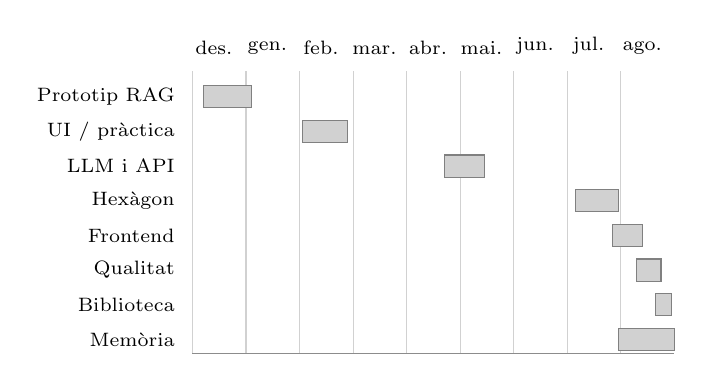
\begin{tikzpicture}[
  font=\scriptsize,
  x=0.68cm, y=0.44cm,
  bar/.style={fill=black!18, draw=black!50, thin},
]
\foreach \x/\m in {0/des.,1/gen.,2/feb.,3/mar.,4/abr.,5/mai.,6/jun.,7/jul.,8/ago.} {
  \node[anchor=south] at (3.3+\x+0.4, 8.45) {\m};
  \draw[black!18] (3.3+\x, 0.1) -- (3.3+\x, 8.25);
}
\draw[black!45] (3.3,0.1) -- (12.3,0.1);
\providecommand{\tfmganttbar}[4]{%
  \node[anchor=east, align=right] at (3.15,#1) {#4};
  \fill[bar] (3.3+#2,#1-0.32) rectangle (3.3+#3,#1+0.32);
}
\tfmganttbar{7.5}{0.2}{1.1}{Prototip RAG}
\tfmganttbar{6.5}{2.05}{2.9}{UI / pràctica}
\tfmganttbar{5.5}{4.7}{5.45}{LLM i API}
\tfmganttbar{4.5}{7.15}{7.95}{Hexàgon}
\tfmganttbar{3.5}{7.85}{8.4}{Frontend}
\tfmganttbar{2.5}{8.3}{8.75}{Qualitat}
\tfmganttbar{1.5}{8.65}{8.95}{Biblioteca}
\tfmganttbar{0.5}{7.95}{9.0}{Memòria}
\end{tikzpicture}

\caption{Diagrama de Gantt simplificat (desembre 2025 -- agost 2026). Els buits (sobretot març i juny) són pauses reals de Git, no sprints continus.}
\label{fig:gantt}
\end{figure}

A 25\,€/hora (tarifa acadèmica habitual en TFM, no de mercat), el cost estimat de la dedicació és de \textbf{9.750\,€}. El projecte és de recerca i aprenentatge, no d'explotació comercial: un pas a producció (allotjament, quotes d'API, manteniment) quedaria fora d'aquest pressupost. El cost variable d'API (embeddings i xat) és a la secció~\ref{sec:cost-api}. El detall de fases d'enginyeria es reprèn al capítol~\ref{cap:gestion}.

\section{Estructura de la memòria}

El capítol~\ref{cap:arte} situa el treball a la literatura. El~\ref{cap:requisitos} fixa requisits. Els capítols~\ref{cap:arquitectura} i~\ref{cap:desarrollo} descriuen disseny i implementació de l'estat actual del repositori. El~\ref{cap:resultados} defineix l'avaluació. El~\ref{cap:gestion} cobreix planificació, riscos i ètica. El~\ref{cap:conclusiones} tanca amb conclusions i línies futures.
